\documentclass[aspectratio=169]{beamer}
\usetheme{Madrid}
\usecolortheme{default}
\usepackage[utf8]{inputenc}
\usepackage{listings}
\usepackage{tikz}
\usepackage{booktabs}
\setbeamertemplate{navigation symbols}{}

\title[Beamer Demo]{Presentations with Beamer}
\subtitle{Technical Writing Class}
\author{Suraj Pathak}
\institute[MNIT]{MNIT Jaipur}
\date{\today}

\lstset{basicstyle=\ttfamily\footnotesize, frame=single, breaklines=true}

\begin{document}

\begin{frame}
  \titlepage
\end{frame}

\begin{frame}{Outline}
  \tableofcontents
\end{frame}

\section{Basics}
\begin{frame}{What is Beamer?}
  Beamer is a \LaTeX{} class for slide presentations.
  \begin{itemize}
    \item Slides are written as plain text
    \item Produces a PDF
    \item Same tools as \LaTeX{}: math, tables, code
  \end{itemize}
\end{frame}

\begin{frame}{Overlays}
  \begin{enumerate}
    \item<1-> Shown from the first click
    \item<2-> Appears on the second
    \item<3-> Appears on the third
  \end{enumerate}
  \only<4>{\alert{Only visible on step 4.}}
\end{frame}

\section{Content}
\begin{frame}{Blocks}
  \begin{block}{Definition}
    A commit is a recorded snapshot of the project.
  \end{block}
  \begin{alertblock}{Warning}
    Never commit passwords or tokens.
  \end{alertblock}
  \begin{exampleblock}{Example}
    \texttt{git commit -m "Add feature"}
  \end{exampleblock}
\end{frame}

\begin{frame}{Columns}
  \begin{columns}
    \column{0.5\textwidth}
    \textbf{Git}
    \begin{itemize}
      \item Version control
      \item Works locally
    \end{itemize}
    \column{0.5\textwidth}
    \textbf{GitHub}
    \begin{itemize}
      \item Hosting platform
      \item Pull requests
    \end{itemize}
  \end{columns}
\end{frame}

\begin{frame}{Math and Tables}
  \[ \int_0^1 x^2\,dx = \frac{1}{3} \]
  \begin{tabular}{lr}
    \toprule
    Tool & Purpose \\
    \midrule
    Beamer & Slides \\
    Doxygen & Code docs \\
    \bottomrule
  \end{tabular}
\end{frame}

\begin{frame}[fragile]{Code}
\begin{lstlisting}[language=C++]
#include <iostream>
int main() {
    std::cout << "Hello";
    return 0;
}
\end{lstlisting}
\end{frame}

\begin{frame}{Graphics with TikZ}
  \centering
  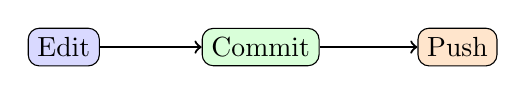
\begin{tikzpicture}[node distance=2.5cm]
    \node[draw,rounded corners,fill=blue!15] (a) {Edit};
    \node[draw,rounded corners,fill=green!15,right of=a] (b) {Commit};
    \node[draw,rounded corners,fill=orange!20,right of=b] (c) {Push};
    \draw[->,thick] (a) -- (b);
    \draw[->,thick] (b) -- (c);
  \end{tikzpicture}
\end{frame}

\section{Summary}
\begin{frame}{Summary}
  \begin{itemize}
    \item One \texttt{frame} per slide
    \item Use blocks, columns and overlays for structure
    \item Choose a theme with \texttt{\textbackslash usetheme\{...\}}
  \end{itemize}
  \centering \Large Thank you!
\end{frame}

\end{document}
